\comment{https://www.youtube.com/watch?v=sgQAhG5Q7iY}

The research sources and  methods are discussed in the following subsections.

The proposed system is divided into three major components shown in \figurename~\ref{fig:sytem-overview} which includes the web client, web server and machine learning models. The web interface get the user health data and sends it to the web server for processing. The web server passes the data to the trained model and returns the binary output which the user sees.

\begin{figure}[htb]
	\centering
	\makebox[0cm]{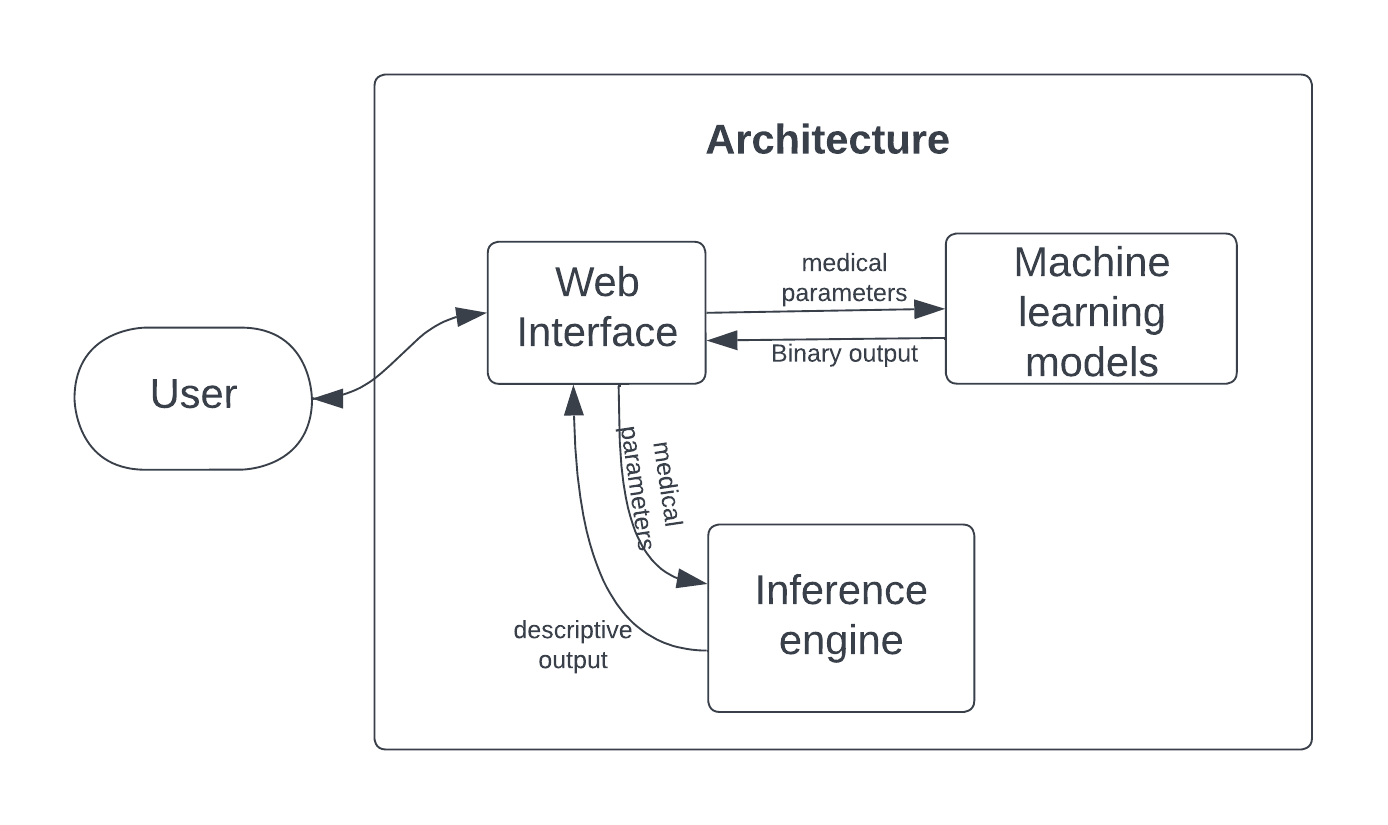
\includegraphics[scale=0.8]{system-overview.png}}
	\caption{System overview}
	\label{fig:sytem-overview}
\end{figure}


\section{Machine learning workflow}
\figurename~\ref{fig:ml-workflow} shows the workflow of for creating the machine learning model.

\begin{figure}[htb]
	\centering
	\makebox[0cm]{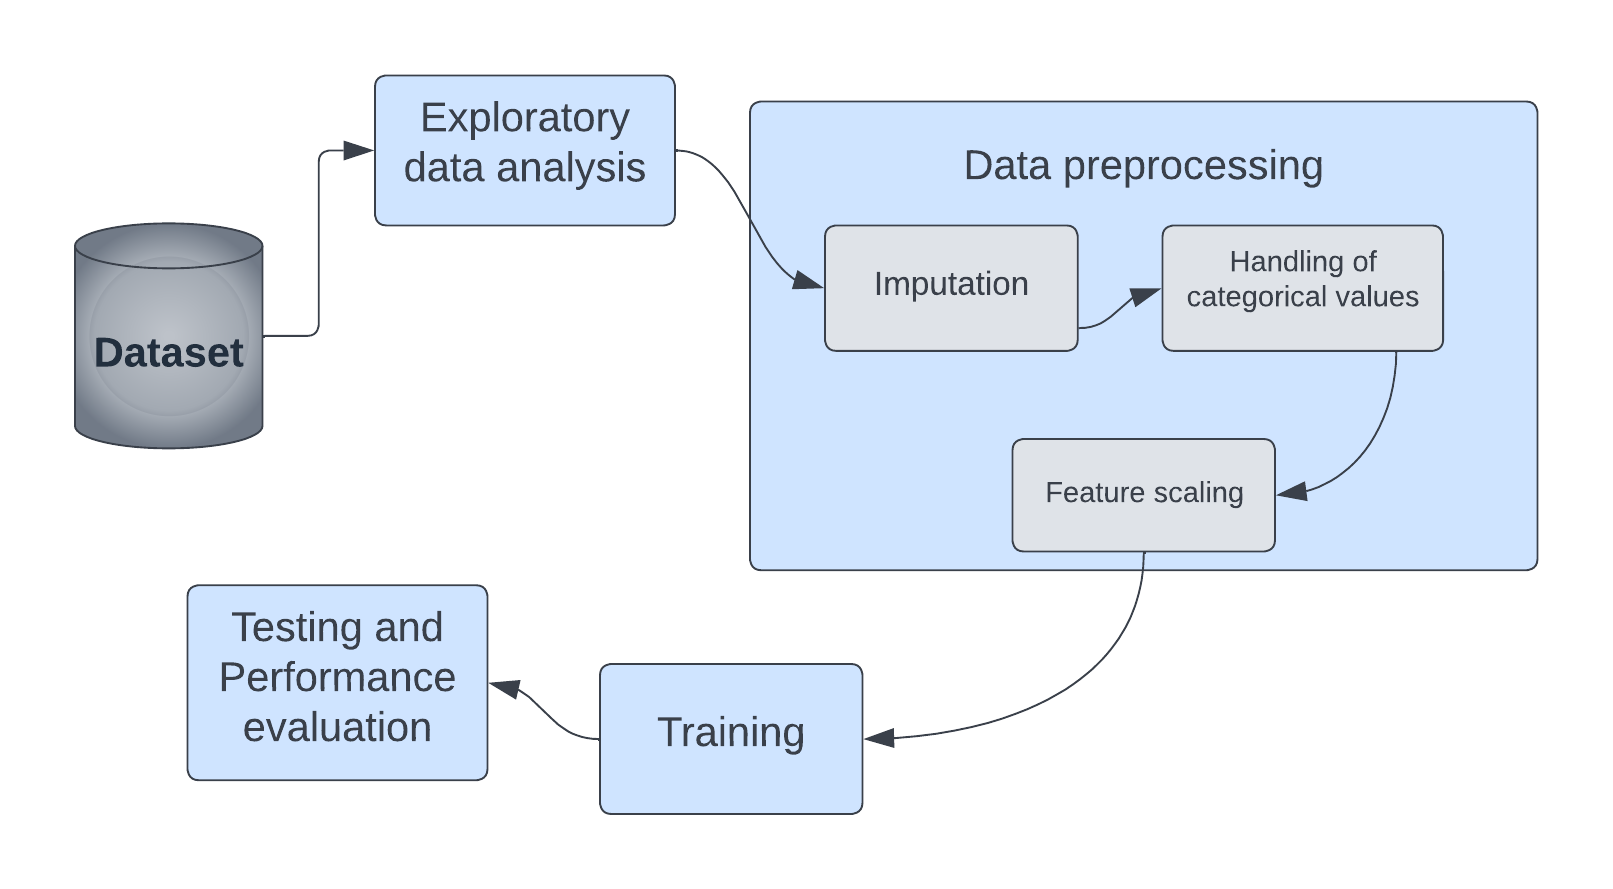
\includegraphics[scale=0.6]{ml-workflow.png}}
	\caption{Machine learning workflow}
	\label{fig:ml-workflow}
\end{figure}

\subsection{Dataset}
An estimated 17.9 million people die each year as a result of cardiovascular diseases (CVDs), making up 31\% of all deaths worldwide. Heart attacks and strokes are the cause of mortality for three-quarters of people under the age of 70 who die from CVD. Several CVDs can lead to heart failure, and this dataset comprises 11 variables that can be used to gauge the likelihood of heart failure.

An early diagnosis and management strategy can be of significant use to people with coronary heart disease or those at high risk of developing the illness because of the existence of risk factors such as hypertension, diabetes, and hyperlipidaemia.

\subsubsection{Features}
These features represent the different columns in the dataset
\begin{itemize}
	\item{\textbf{Age:} age of the patient [years]}
	\item{\textbf{Sex:} sex of the patient [M: Male, F: Female]}
	\item{\textbf{ChestPainType:} chest pain type [TA: Typical Angina, ATA: Atypical Angina, NAP: Non-Anginal Pain, ASY: Asymptomatic]}
	\item{\textbf{RestingBP:} resting blood pressure [mm Hg]}
	\item{\textbf{Cholesterol:} serum cholesterol [mm/dl]}
	\item{\textbf{FastingBS:} fasting blood sugar [1: if FastingBS $>$ 120 mg/dl, 0: otherwise]}
	\item{\textbf{RestingECG:} resting electrocardiogram results [Normal: Normal, ST: having ST-T wave abnormality (T wave inversions and/or ST elevation or depression of > 0.05 mV), LVH: showing probable or definite left ventricular hypertrophy by Estes' criteria]}
	\item{\textbf{MaxHR:} maximum heart rate achieved [Numeric value between 60 and 202]}
	\item{\textbf{ExerciseAngina:} exercise-induced angina [Y: Yes, N: No]}
	\item{\textbf{Oldpeak:} oldpeak = ST [Numeric value measured in depression]}
	\item{\textbf{ST\textunderscore Slope:} the slope of the peak exercise ST segment [Up: upsloping, Flat: flat, Down: downsloping]}
	\item{\textbf{HeartDisease}:output class [1: heart disease, 0: Normal]}
\end{itemize}

\subsubsection{Target variable}
In the context of machine learning, the term "target variable" refers to the variable that either is or should be the output. If you are classifying the data, for instance, it could be a binary 0 or 1, but if you are running a regression, it could be a continuous variable. In the field of statistics, this concept is also known as the response variable.

In the context of this research, the variable HeartDisease serves as our target variable. We are interested in identifying whether or not somebody is likely to get heart disease based on the input parameters such as gender, age, and the results of numerous tests.

\subsection{Exploratory data analysis}
Exploratory data analysis, (EDA) is the important process of looking at data for the first time to find patterns, find outliers, test hypotheses, and check assumptions with the help of summary statistics and graphical representations. This is done to make sure that the data are correct and can be reliable. 

\subsubsection{Why do we need EDA?}
The reasons for perfoming EDA are summarized below:

\begin{enumerate}
	\item Understanding the dataset helps clean up the dataset.
	\item It gives a clear idea of the features and how they fit together.
	\item Gives guidelines for what variables are important and what variables can be left out or taken away.
	\item Handling Missing values or human error.
	\item Identifying outliers.
	\item The EDA process would help to get the most information out of a dataset.
	\item EDA takes time but its very effective.
\end{enumerate}

\subsection{Data preprocessing}
Data preprocessing is required for accurate data representation and machine learning classifiers, for proper training and evaluation. For the dataset to be used effectively by the classifiers, preprocessing methods such imputation, feature scaling and handling of categorical variable have been applied.

\subsubsection{Imputation}
Imputation is a straightforward operation that involves replacing the values in our dataset that are absent (null). We can accomplish this by implementing our own specialized function, or we can simply perform imputation by making use of sklearn's built-in SimpleImputer class. Both of these options are available to use. For example:
\begin{lstlisting}[language=Python, numbers=none, label=Simple Imputer]
	from sklearn.impute import SimpleImputer
	
	imputer = SimpleImputer(missing_values=np.nan, strategy='mean')
	imputer = imputer.fit(df[['Weight']])
	df['Weight'] = imputer.transform(df[['Weight']])
\end{lstlisting}

\subsubsection{Feature scaling}

Feature scaling is a method for uniformly reducing the values of each independent feature in our dataset. Algorithms can be calculated much more quickly with the aid of feature scaling making it a significant step in the preprocessing of data. The machine learning models would give larger weights to higher values and lower weights to lower values if we hadn't scaled the features. Additionally, training the machine learning model will take a longer time without scaling. The standard scalar is a feature scaling method that guarantees that they all have the same mean and variance. Although there were no features with missing values in the dataset, it is a recommended practice to check for and remove data units with missing values. These data preprocessing methods were all applied in this study.

\subsubsection{Handling of categorical variables}
Categorical variables/features are any feature type can be classified into two major types:
\begin{itemize}
	\item Nominal
	\item Ordinal
\end{itemize}
Nominal variables are those that have two or more categories that are not in any particular order. For example, gender can be thought of as a nominal variable if it is split into two groups, male and female. On the other hand, ordinal variables have "levels" or categories that are in a certain order. For example, an ordinal categorical variable can be a feature with three levels: low, medium, and high. Order is important.

This is a binary classification problem, and although the target is not skewed, we apply the best metric for it, which is the area under the ROC curve (AUC). Although precision and recall are also options, AUC combines precision and recall. As a result, we will use AUC to assess the model that we create using this dataset.

Since text data cannot be understood by computers, we must transform these categories to numbers. This may be done easily by using:

\begin{itemize}
	\item{Label Encoding: using sklearn's LabelEncoder class}
	\begin{lstlisting}[language=Python, caption=Label Encoder, numbers=none]
	from sklearn.preprocessing import LabelEncoder\end{lstlisting}
	\item{One Hot Encoding: using pandas get\_dummies method on the dataframe.}
	\begin{lstlisting}[language=Python, caption=Get dummies, numbers=none]
	pd.get_dummies()\end{lstlisting}
\end{itemize}
But we must know when to apply which kind of label encoding: \\
\\
\noindent
\textbf{One-Hot Encoding is the best use for non-tree based Machine Learning Algorithms.}
\begin{itemize}
	\item The advantage of One-Hot-Encoding is that the result is binary rather than ordinal and that everything is in an orthogonal vector space.
	\item The negative is that with large cardinality, the feature space can quickly explode and you are forced to deal with the curse of dimensionality. In these circumstances, I usually use one-hot encoding followed by PCA to reduce dimensionality. Other encoding strategies rarely outperform the prudent combination of one-hot plus PCA, in my opinion. Because PCA detects linear overlap, it will naturally group comparable features together.
\end{itemize}

\noindent
\textbf{For three based algorithms, label encoding is the best way to go.}

\begin{itemize}
	\item{LabelEncoder can convert [dog,cat,dog,mouse,cat] to [1,2,1,3,2], however the required ordinality means that cat is the average of dog and mouse. There are still algorithms that operate well with categorical variables, such as decision trees and random forests, and LabelEncoder can be used to store values with minimal disk space.}
\end{itemize}

\comment{

\subsubsection{Cross validation \& Hyperparameter optimisation}
In machine learning, choosing the best hyperparameters for a learning algorithm is called hyperparameter optimization or tuning. It is possible to regulate the learning process by altering a parameter's value, which is known as a hyperparameter. It's a different case when it comes to learning other parameters (usually node weights).
1
The same machine learning model may need various constraints, weights, or rates of learning to generalize to diverse patterns of input data. These parameters, also known as hyperparameters, must be fine-tuned to ensure that the model is able to tackle the machine learning problem to its full potential. To minimize a predetermined loss function on provided independent data, a hyperparameter optimization model is constructed by finding a pair of hyperparameters that minimizes the loss function. The loss associated with a tuple of hyperparameters is returned by the objective function. As a generalization test, cross-validation is commonly utilized.
}

\subsection{Training the models}
The following machine learning algorithms will be used for building the classification model.

\subsubsection{Cross validation}
In cross-validation, training data is split into a few parts. Some of these parts are used to train the model, and the rest are used to test it.

The best cross-validation method to use will depend on the dataset you are working with, and it may or may not be applicable to other datasets. There are a few cross-validation techniques, though, that are the most well-known and frequently employed. These consist of:

\begin{enumerate}
	\item K-fold cross-validation.
	\item Stratified k-fold cross-validation
\end{enumerate}

You shouldn't use random k-fold cross-validation if you have a skewed dataset for binary classification with 90\% positive samples and only 10\% negative samples. If you use simple k-fold cross-validation on a set of data like this, you might end up with folds that have no positive samples at all. We like to use stratified k-fold cross-validation in these situations. The number of labels in each fold stays the same with stratified k-fold cross-validation. So, you will have the same 90\% positive and 10\% negative samples in each fold. So, no matter what metric you use to measure, the results will be the same for all folds. So in the case, we would be using stratified k-fold cross-validation technique.

\subsubsection{Logistic regression}
Classification algorithms, such as logistic regression, are supervised.
This statistical model is frequently employed in categorization and predictive analytics. Based on a collection of independent variables, logistic regression calculates the likelihood that a certain event will occur. 

As a result, the dependent variable is limited to a range of 0 to 1. 
Independent variables are analysed to determine the binary outcome with the results falling into one of two categories. The independent variables can be categorical or numeric, but the dependent variable is always categorical. Written like this: $$P(Y=1|X) or P(Y=0|X)$$
It calculates the probability of dependent variable Y, given independent variable X. 

\comment{
It calculates the probability of dependent variable Y, given independent variable X.

This can be used to calculate the probability of a word having a positive or negative connotation (0, 1, or on a scale between). Or it can be used to determine the object contained in a photo (tree, flower, grass, etc.), with each object given a probability between 0 and 1.
}



\subsubsection{Naive Bayes}

Naïve bayes is a machine learning algorithm used to solve classification problems. Naïve bayes is based on the Bayes Theorem and is one of the simplest yet powerful ML algorithms in use. It finds applications in many industries.

The Bayes' theorem is used by Naïve Bayes algorithm, which also assumes that each predictor is independent. To put it another way, this classifier makes the assumption that the presence of one specific feature in a class has no influence on the presence of another.

\begin{figure}[htb]
	\centering
	\makebox[0cm]{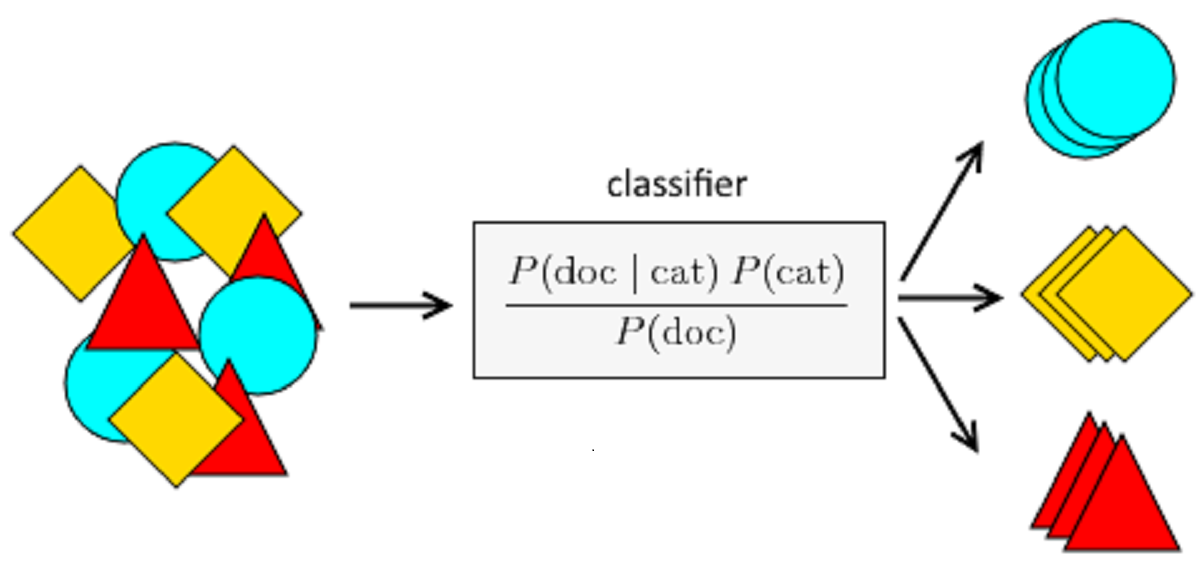
\includegraphics[scale=0.5]{nb.png}}
	\caption{Naive bayes}
	\label{fig:nb}
\end{figure}


\subsubsection{K-nearest neighbours}
The K-nearest neighbors (KNN) algorithm is a form of supervised learning technique that can be used for regression as well as classification. KNN performs a distance calculation between the test data and all of the training points in an effort to determine which class the data being evaluated should be assigned to. The K number of points that should be selected is the one that comes closest to the test data. The KNN algorithm computes the chance that the test data belong to the same classes as the 'K' training data, and the class that retains the highest probability is the one that is chosen. In the case of regression, the value is determined by calculating the average of the 'K' training points that were chosen.
\\

Let's say we have a picture of something that looks like both a cat and a dog, but we want to know if it's a cat or a dog. We can use the KNN method for this identification because it measures similarity. Our KNN model will look for similarities between the new data set and the images of cats and dogs. Based on the similarities it finds, it will put the new data set into either the cat or dog category.

\begin{figure}[htb]
	\centering
	\makebox[0cm]{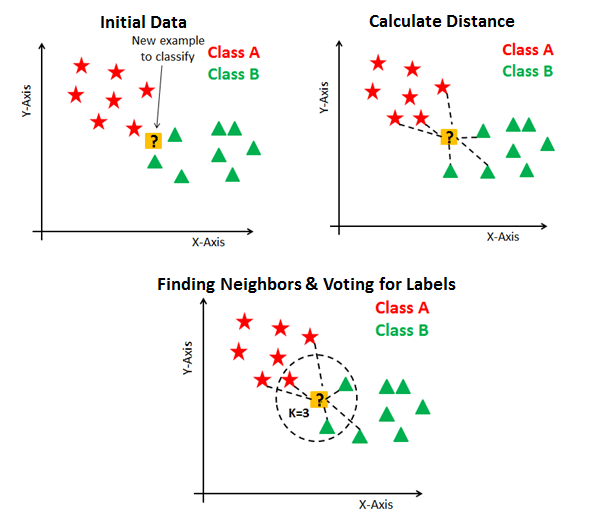
\includegraphics[scale=0.45]{KNN.png}}
	\caption{K-nearest neighbours}
	\label{fig:knn}
\end{figure}

\subsubsection{Decision Tree}
A decision tree is a non-parametric supervised learning algorithm that can be used for both classification and regression tasks. As a supervised learning technique, a decision tree is ideal for classifying issues at a precise level of detail. Like a flow chart, it takes data from the "tree trunk" and divides it into two related categories at a time: "branches" and "leaves." This allows for organic classification with minimal human oversight by creating categories within categories.

\comment{
	\begin{figure}[htb]
		\centering
		\makebox[0cm]{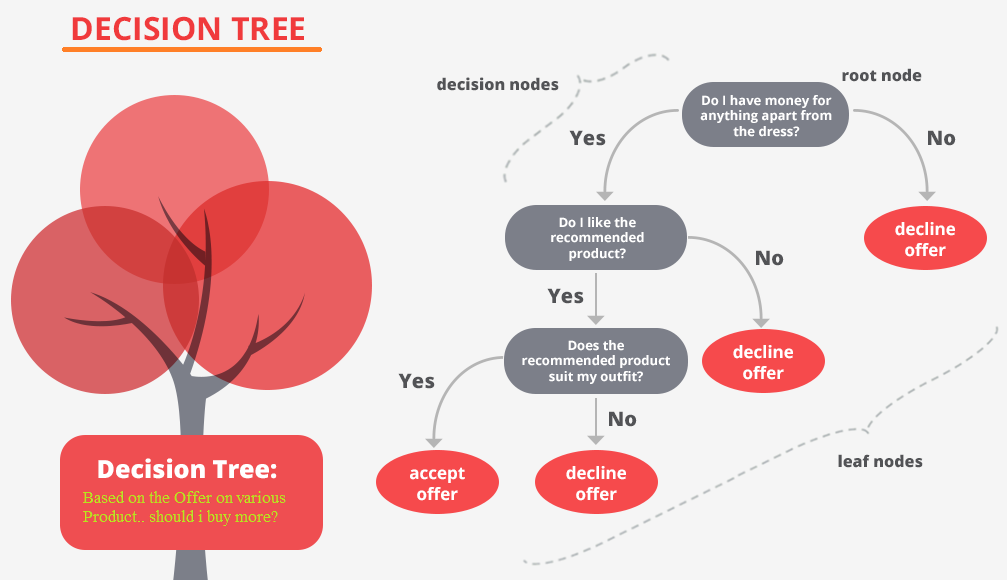
\includegraphics[scale=0.45]{dt.png}}
		\caption{Decision tree}
		\label{fig:dt}
	\end{figure}
}

\subsection{Performance evaluation}
When it comes to classification problems, the following measures are most frequently used:

\begin{itemize}
	\item{Accuracy}
	\item{Precision (P)}
	\item{Recall (R)}
	\item{F1 score (F1)}
	\item{Area under the ROC (Receiver Operating Characteristic) curve or simply AUC (AUC)
		\begin{itemize}
			\item {When you have a dataset with skewed binary targets, another measure that is frequently employed is the area under the ROC curve calculation. The Area Under ROC Curve, Area Under Curve, or plain AUC are all names for this measure. The area under the ROC curve can be calculated in a variety of methods.}
			\item{AUC is a metric that is frequently used in machine learning for skewed binary classification tasks.}
		\end{itemize}
	}
\end{itemize}

\section{Web interface}
The web interface consists of the web server and client components that provides a way for users to interact with the machine learning algorithms.

\begin{figure}[htb]
\centering
\makebox[0cm]{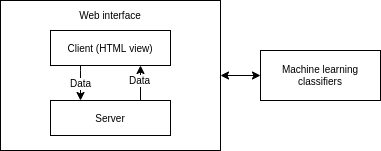
\includegraphics[scale=0.8]{web-interface.png}}
\caption{Web interface}
\label{fig:web-interface}
\end{figure}

A web server is software and hardware that responds to client requests sent over the World Wide Web using the HTTP (Hypertext Transfer Protocol) and other protocols. A web server's primary responsibility is to show website content by storing, processing, and sending webpages to users.

The web server is built in python with the python \href{https://flask.palletsprojects.com/en/2.1.x/}{flask} web framework using \href{https://jinja.palletsprojects.com/en/3.1.x/}{jinja} as a templating engine for the client interface. The server extracts the input data from a form the user submits via a post endpoint and validates the data so there is no invalid input. The implementations of the server will be discussed in \autoref{chap:4}.

\begin{figure}[htb]
	\centering
	\makebox[0cm]{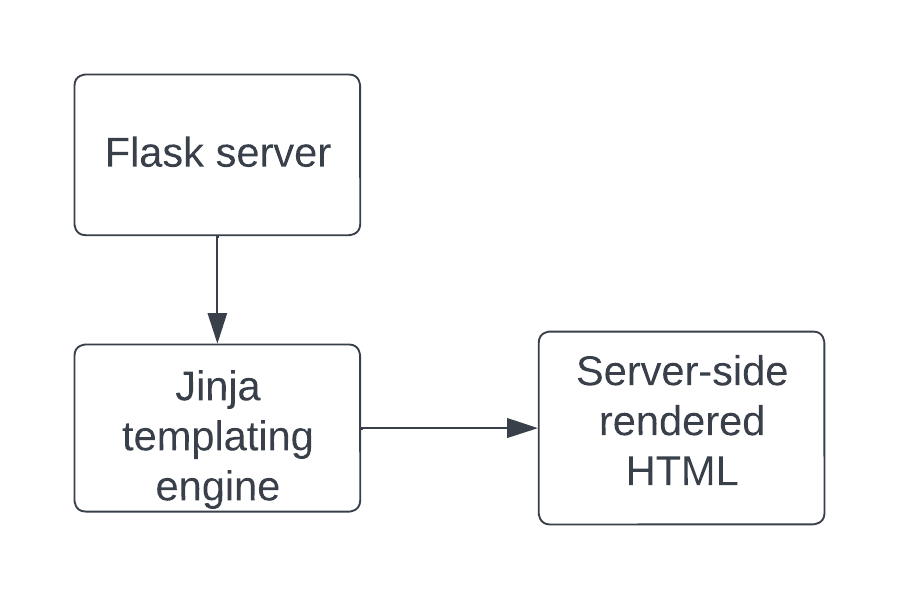
\includegraphics[scale=0.8]{server.png}}
	\caption{Server}
	\label{fig:server}
\end{figure}